% Created 2024-09-15 Sun 15:05
% Intended LaTeX compiler: pdflatex
\documentclass[11pt]{article}
\usepackage[utf8]{inputenc}
\usepackage[T1]{fontenc}
\usepackage{graphicx}
\usepackage{longtable}
\usepackage{wrapfig}
\usepackage{rotating}
\usepackage[normalem]{ulem}
\usepackage{amsmath}
\usepackage{amssymb}
\usepackage{capt-of}
\usepackage{hyperref}
\author{Jackson Mowry}
\date{Sun Sep 15 15:04:51 2024}
\title{Hw3}
\hypersetup{
 pdfauthor={Jackson Mowry},
 pdftitle={Hw3},
 pdfkeywords={},
 pdfsubject={},
 pdfcreator={Emacs 29.4 (Org mode 9.7.11)}, 
 pdflang={English}}
\begin{document}

\maketitle
\tableofcontents

\section{1}
\label{sec:org8fb3ea7}
\begin{enumerate}
\item \begin{center}
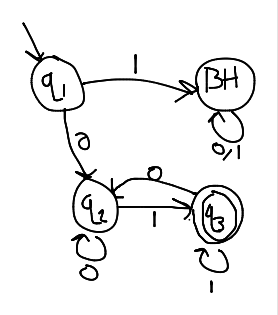
\includegraphics[width=.9\linewidth]{1-1.png}
\end{center}
\end{enumerate}
\begin{center}
\begin{tabular}{l|l|l}
State & 0 & 1\\
\hline
q\textsubscript{1} & q\textsubscript{2} & BH\\
q\textsubscript{2} & q\textsubscript{2} & q\textsubscript{3}\\
q\textsubscript{3} & q\textsubscript{2} & q\textsubscript{3}\\
BH & BH & BH\\
\end{tabular}
\end{center}
q\textsubscript{0} (start) = q\textsubscript{1}
F (accept) = q\textsubscript{3}
\begin{enumerate}
\item \begin{center}
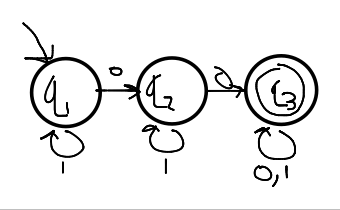
\includegraphics[width=.9\linewidth]{1-2.png}
\end{center}
\end{enumerate}
\begin{center}
\begin{tabular}{l|l|l}
State & 0 & 1\\
\hline
q\textsubscript{1} & q\textsubscript{2} & q\textsubscript{1}\\
q\textsubscript{2} & q\textsubscript{3} & q\textsubscript{2}\\
q\textsubscript{3} & q\textsubscript{3} & q\textsubscript{3}\\
\end{tabular}
\end{center}
q\textsubscript{0} (start) = q\textsubscript{1}
F (accept) = q\textsubscript{3}
\begin{enumerate}
\item \begin{center}
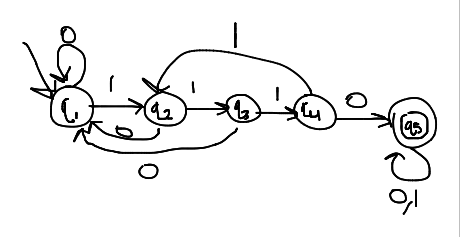
\includegraphics[width=.9\linewidth]{1-3.png}
\end{center}
\end{enumerate}
\begin{center}
\begin{tabular}{l|l|l}
State & 0 & 1\\
\hline
q\textsubscript{1} & q\textsubscript{1} & q\textsubscript{2}\\
q\textsubscript{2} & q\textsubscript{1} & q\textsubscript{3}\\
q\textsubscript{3} & q\textsubscript{1} & q\textsubscript{4}\\
q\textsubscript{4} & q\textsubscript{5} & q\textsubscript{2}\\
q\textsubscript{5} & q\textsubscript{5} & q\textsubscript{5}\\
\end{tabular}
\end{center}
q\textsubscript{0} (start) = q\textsubscript{1}
F (accept) = q\textsubscript{5}
\section{2}
\label{sec:org17b8d96}
\begin{center}
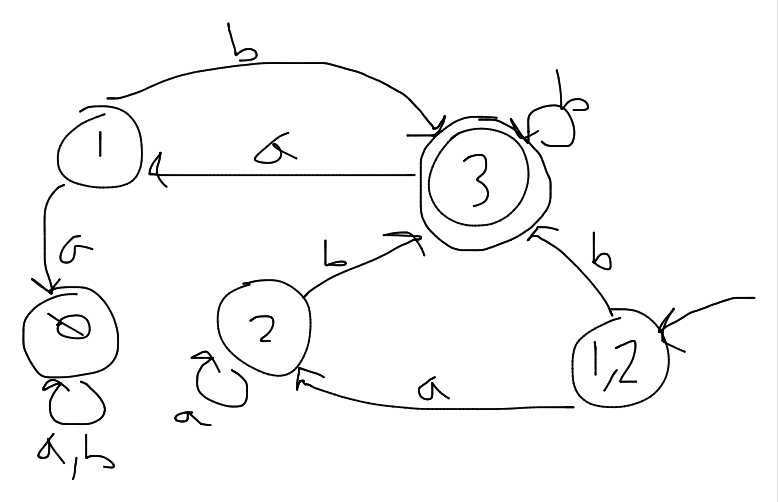
\includegraphics[width=.9\linewidth]{2.png}
\end{center}
\begin{center}
\begin{tabular}{r|r|r}
State & a & b\\
0 & 0 & 0\\
1 & 0 (Black Hole) & 3\\
2 & 2 & 3\\
3 & 1 & 3\\
1,2 & 2 & 3\\
\end{tabular}
\end{center}
q\textsubscript{0} (start) = 1,2
F (accept) = 3
\end{document}
